\documentclass[11pt,a4paper]{article}

\usepackage[utf8]{inputenc}
\usepackage[brazil]{babel}
\usepackage{lmodern}
\usepackage{amsmath}
\usepackage{amssymb}
\usepackage[top=1.6cm, bottom=1.6cm, left=1.8cm, right=1.8cm]{geometry}
\usepackage{graphicx}
\usepackage{booktabs}
\usepackage{tabularx}
\usepackage{xcolor}
\usepackage{hyperref}
\usepackage{tcolorbox}
\usepackage{fancyhdr}
\usepackage{enumitem}

% Definições de cores institucionais / técnicas
\definecolor{primary}{RGB}{20, 45, 85}
\definecolor{secondary}{RGB}{40, 90, 150}
\definecolor{accent}{RGB}{180, 40, 40}
\definecolor{bglight}{RGB}{245, 247, 250}
\definecolor{bordercolor}{RGB}{200, 210, 225}

\hypersetup{
    colorlinks=true,
    linkcolor=primary,
    urlcolor=secondary,
    citecolor=accent
}

\pagestyle{fancy}
\fancyhf{}
\fancyhead[L]{\small \textbf{IME 04-10842 -- Computação Gráfica} | Trabalho Final 2026.1}
\fancyhead[R]{\small Simulador Formiga Robô 3D}
\fancyfoot[C]{\thepage}

\tcbuselibrary{skins,breakable}

\newtcolorbox{infoBox}[1]{
    colback=bglight,
    colframe=secondary,
    coltitle=white,
    fonttitle=\bfseries,
    title=#1,
    arc=3mm,
    boxrule=1pt,
    left=4mm, right=4mm, top=3mm, bottom=3mm
}

\newtcolorbox{warningBox}[1]{
    colback=white,
    colframe=accent,
    coltitle=white,
    fonttitle=\bfseries,
    title=#1,
    arc=2mm,
    boxrule=1pt,
    left=4mm, right=4mm, top=3mm, bottom=3mm
}

\begin{document}

% ------------------------------------------------------------------------------
% CABEÇALHO / CAPA TÉCNICA
% ------------------------------------------------------------------------------
\begin{center}
    {\large \textbf{INSTITUTO MILITAR DE ENGENHARIA -- IME}}\\[2mm]
    {\large DEPARTAMENTO DE ENGENHARIA ELÉTRICA}\\[2mm]
    {\large DISCIPLINA: COMPUTAÇÃO GRÁFICA (IME 04-10842) -- 2026.1}\\[5mm]
    
    \vspace{2mm}
    \begin{tcolorbox}[colback=primary, colframe=primary, arc=3mm, halign=center]
        \vspace{1mm}
        {\Huge \bfseries \textcolor{white}{MANUAL DE INSTRUÇÕES}}\\[2mm]
        {\Large \bfseries \textcolor{white}{Simulador 3D de Formiga Robô em OpenGL Clássico}}\\[1mm]
        {\normalsize \textcolor{white}{\textit{Anatomia Hierárquica, Cinemática Tripod Gait, Multi-Texturas BMP e Iluminação Metálica}}}
        \vspace{1mm}
    \end{tcolorbox}
    
    \vspace{3mm}
    \textbf{Autor:} Mateus Henrique Freitas Maciel \quad | \quad \textbf{Professor:} Paulo Cezar Pinto Carvalho\\[1mm]
    \textbf{Entrega:} Outubro de 2026 \quad | \quad \textbf{Versão Oficial:} v1.0.0
\end{center}

\vspace{2mm}

% Imagem de Preview se existir
\begin{center}
    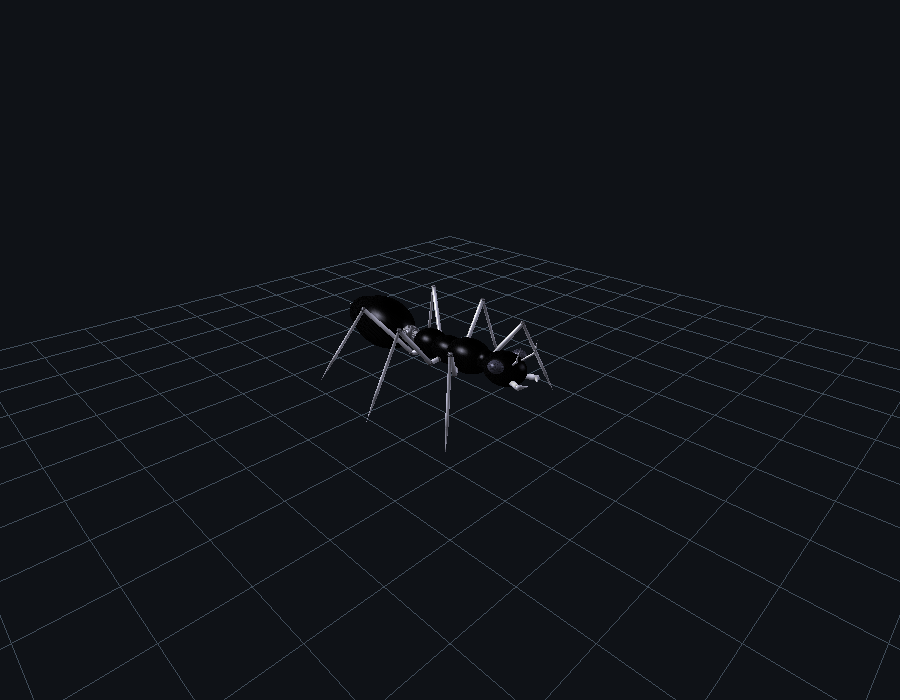
\includegraphics[width=0.48\textwidth]{docs/screenshot_formiga.png}\\[1mm]
    \textit{\footnotesize Figura 1: Renderização em tempo real do Simulador da Formiga Robô com texturas multi-materiais e iluminação metálica.}
\end{center}

\vspace{-2mm}

% ------------------------------------------------------------------------------
% SEÇÃO 1: INSTRUÇÕES DE COMPILAÇÃO E EXECUÇÃO
% ------------------------------------------------------------------------------
\section{Instruções de Compilação e Execução}

O projeto foi rigorosamente desenvolvido utilizando \textbf{apenas C++ padrão, OpenGL clássico (pipeline fixo), GLU, GLUT (FreeGLUT)} e a biblioteca local \texttt{RgbImage} (\texttt{RgbImage.h} e \texttt{RgbImage.cpp}), cumprindo integralmente as exigências do enunciado.

\subsection{Ambiente Linux}
Para compilar e executar no Linux (com \texttt{freeglut3-dev}):
\begin{itemize}[leftmargin=*,noitemsep]
    \item \textbf{Compilação e Execução Direta:} \texttt{make run}
    \item \textbf{Validação Obrigatória (-Wall -Wextra -Werror):} \texttt{make validate}
    \item \textbf{Linha de comando manual:}
    \texttt{g++ -Wall -Wextra -Werror -O2 formiga.cpp RgbImage.cpp -lGL -lGLU -lglut -lm -o formiga}
\end{itemize}

\subsection{Ambiente Windows}
O arquivo \texttt{formiga.cpp} inclui na linha 1 a diretiva \texttt{\#define \_CRT\_SECURE\_NO\_WARNINGS} e a inclusão condicional de \texttt{<windows.h>} antes de \texttt{<GL/glut.h>}:
\begin{itemize}[leftmargin=*,noitemsep]
    \item \textbf{MinGW / GCC (64-bits):}
    \texttt{g++ -O2 formiga.cpp RgbImage.cpp -lfreeglut -lopengl32 -lglu32 -o formiga.exe}
    \item \textbf{Execução:} Certifique-se de que a biblioteca \texttt{freeglut.dll} (fornecida) e as texturas estejam no mesmo diretório do executável \texttt{formiga.exe}.
\end{itemize}

\newpage

% ------------------------------------------------------------------------------
% SEÇÃO 2: TABELA COMPLETA DE COMANDOS INTERATIVOS
% ------------------------------------------------------------------------------
\section{Tabela Completa de Comandos Interativos}

A interação do usuário com o simulador ocorre de forma integrada via teclado e mouse:

\begin{table}[h!]
\centering
\small
\begin{tabularx}{\textwidth}{l p{4.8cm} X}
\toprule
\textbf{Entrada} & \textbf{Ação / Movimento} & \textbf{Descrição Funcional} \\
\midrule
\multicolumn{3}{l}{\textbf{\textcolor{primary}{1. Controles da Câmera (Projeção Perspectiva e Viewport)}}} \\
\midrule
\textbf{Mouse Esquerdo + Arraste} & Rotação Orbital 360° & Órbita esférica contínua ao redor do robô (azimute e elevação). \\
\textbf{Mouse Direito + Arraste} & Pan da Câmera & Translação suave do ponto focal no plano de visualização. \\
\textbf{Scroll do Mouse} ou \textbf{+ / -} & Zoom In / Zoom Out & Aproxima e afasta a câmera sem distorção projetiva. \\
\textbf{Setas Teclado} & Órbita via Teclado & Esquerda/Direita (azimute) e Cima/Baixo (elevação). \\
\textbf{W / S / A / D} & Navegação Clássica & Compatibilidade direta com os controles legados de \texttt{garra.cpp}. \\
\textbf{I / K} & Pan Vertical Teclado & Eleva ou abaixa o alvo focal da câmera. \\
\textbf{R / r} & Reset Geral & Restaura a câmera padrão, zera articulações e para a caminhada. \\
\midrule
\multicolumn{3}{l}{\textbf{\textcolor{primary}{2. Locomoção Automática da Formiga}}} \\
\midrule
\textbf{Barra de Espaço} & \textbf{Caminhada Tripod Gait} & \textbf{Ativa / Desativa a marcha automática de 6 patas a 60 FPS.} \\
\midrule
\multicolumn{3}{l}{\textbf{\textcolor{primary}{3. Articulação Manual das 6 Patas (Braços Mecânicos)}}} \\
\midrule
\textbf{1 / 2} & Articulação da Coxa (Yaw) & Avança (+Yaw) ou recua (-Yaw) horizontalmente as patas. \\
\textbf{3 / 4} & Articulação do Fêmur (Pitch) & Eleva (+Pitch) ou abaixa (-Pitch) os joelhos das 6 patas. \\
\textbf{5 / 6} & Articulação da Tíbia (Pitch) & Flexiona (+Pitch) ou estende (-Pitch) as tíbias em direção ao chão. \\
\midrule
\multicolumn{3}{l}{\textbf{\textcolor{primary}{4. Cabeça e Apêndices Frontais}}} \\
\midrule
\textbf{H / h} & Pitch da Cabeça & Inclina a cabeça verticalmente para cima (\texttt{h}) ou baixo (\texttt{H}). \\
\textbf{Y / y} & Yaw da Cabeça & Gira o pescoço horizontalmente para esquerda (\texttt{y}) ou direita (\texttt{Y}). \\
\textbf{J / j} & Mandíbulas em Pinça & Abre (\texttt{j}) ou fecha (\texttt{J}) as mandíbulas (com trava física sem cruzar). \\
\textbf{U / u} & Antenas Articuladas & Eleva (\texttt{u}) ou abaixa (\texttt{U}) as antenas bi-articuladas no cotovelo. \\
\midrule
\multicolumn{3}{l}{\textbf{\textcolor{primary}{5. Abdômen, Ferrão e Renderização}}} \\
\midrule
\textbf{B / b} & Pitch do Abdômen/Gáster & Eleva (\texttt{b}) ou curva o ferrão para baixo (\texttt{B}) em pose de ataque. \\
\textbf{N / n} & Yaw do Abdômen & Move o abdômen lateralmente para a esquerda (\texttt{n}) ou direita (\texttt{N}). \\
\textbf{T / t} & Alternância de Textura & Liga / Desliga o mapeamento de texturas BMP em tempo real. \\
\textbf{P / p} & Captura de Tela & Salva um screenshot BMP 24-bits em \texttt{docs/screenshot\_formiga.bmp}. \\
\textbf{ESC} & Sair & Encerra o simulador e desaloca recursos de vídeo. \\
\bottomrule
\end{tabularx}
\end{table}

% ------------------------------------------------------------------------------
% SEÇÃO 3: ANATOMIA E MODELAGEM HIERÁRQUICA
% ------------------------------------------------------------------------------
\section{Anatomia da Formiga e Grafo de Cena (Hierarquia de Referenciais)}

A modelagem tridimensional foi estruturada como uma árvore de referenciais cinemáticos (grafo de cena), garantindo que movimentos de nós ancestrais se propaguem automaticamente para seus filhos via pilha matricial (\texttt{glPushMatrix} / \texttt{glPopMatrix}):

\begin{itemize}[leftmargin=*]
    \item \textbf{Tórax (Nó Raiz):} Segmentado anatomicamente em 3 esferoides proporcionais: \textit{Protórax} (anterior, $Y = +0.85$), \textit{Mesotórax} (central, $Y = -0.05$) e \textit{Metatórax} (posterior, $Y = -0.90$).
    \item \textbf{Cabeça e Apêndices:} Conectada ao Protórax por junta esférica de pescoço com 2 graus de liberdade (Pitch e Yaw). Contém crânio proporcional, 2 olhos compostos hemisféricos laterais, 2 mandíbulas horizontais em pinça com dentes curvados para dentro, e 2 antenas bi-articuladas geniculadas (haste basal escapo + cotovelo esférico + flagelo terminal).
    \item \textbf{Cintura e Abdômen (Gáster):} Conectada ao Metatórax por uma dupla cintura articulada (\textit{Pecíolo} e \textit{Pós-Pecíolo}) com rotação em Pitch e Yaw, seguida pelo bulbo do Gáster em formato de gota e um ferrão mecânico cônico.
    \item \textbf{Seis Pernas Articuladas (Cadeias Cinemáticas / Braços Mecânicos):}
    Cada perna é ligada anatomicamente ao seu respectivo segmento torácico:
    \begin{itemize}[noitemsep]
        \item \textbf{Pernas Dianteiras ($L_1 / R_1$):} Conectadas ao Protórax ($Y = +0.80$, inclinação base $+38^\circ$ para frente).
        \item \textbf{Pernas Médias ($L_2 / R_2$):} Conectadas ao Mesotórax ($Y = -0.05$, inclinação base $-10^\circ$).
        \item \textbf{Pernas Traseiras ($L_3 / R_3$):} Conectadas ao Metatórax ($Y = -0.85$, inclinação base $-55^\circ$ para trás, sendo as mais longas).
    \end{itemize}
    Cada perna possui 4 elos em série encadeados puramente ao longo do eixo local $+Z$ (padrão \texttt{garra.cpp}):
    \textit{Junta do Quadril} $\to$ \textit{Segmento Coxa} $\to$ \textit{Junta Trocanter} $\to$ \textit{Segmento Fêmur} $\to$ \textit{Junta Joelho} $\to$ \textit{Segmento Tíbia} $\to$ \textit{Garra Cônica (Tarso)}. Todas as 6 garras tocam simultaneamente o plano de apoio em $Z = -1.65$.
\end{itemize}

\newpage

% ------------------------------------------------------------------------------
% SEÇÃO 4: CINEMÁTICA DA CAMINHADA (TRIPOD GAIT)
% ------------------------------------------------------------------------------
\section{Cinemática da Caminhada: Marcha em Tripé (Tripod Gait)}

Para simular a locomoção real dos hexápodes com máxima estabilidade dinâmica, foi implementada a marcha em tripé alternado (\textit{Alternating Tripod Gait}), garantindo que em qualquer instante haja sempre 3 patas apoiadas no solo formando um triângulo de suporte estático, enquanto as outras 3 avançam pelo ar:

\begin{itemize}[leftmargin=*]
    \item \textbf{Tripé A (Fase $\phi_A = t$):} Dianteira Esquerda ($L_1$), Média Direita ($R_2$) e Traseira Esquerda ($L_3$).
    \item \textbf{Tripé B (Fase $\phi_B = t + \pi$):} Dianteira Direita ($R_1$), Média Esquerda ($L_2$) e Traseira Direita ($R_3$).
\end{itemize}

\textbf{Equações Cinemáticas Contínuas a 60 FPS (Timer de 16 ms):}
\begin{enumerate}[leftmargin=*,noitemsep]
    \item \textbf{Avanço/Recuo da Coxa (Horizontal Yaw):} $\theta_{\text{coxa}} = -A_{\text{coxa}} \cdot \cos(\phi)$. Na fase de balanço no ar ($\sin \phi > 0$), a coxa viaja para frente; no solo ($\sin \phi \le 0$), a coxa empurra o chão para trás.
    \item \textbf{Elevação do Joelho (Vertical Pitch do Fêmur):} Quando $\sin \phi > 0$ (no ar), o fêmur sobe $\theta_{\text{femur}} = A_{\text{femur}} \cdot \sin(\phi)$ descolando a garra do solo. No solo ($\sin \phi \le 0$), $\theta_{\text{femur}} = 0$, mantendo a garra cravada exatamente no plano $Z = -1.65$.
    \item \textbf{Flexão da Tíbia:} No ar, a tíbia flexiona suavemente para evitar colisão com a grade de referência.
\end{enumerate}

% ------------------------------------------------------------------------------
% SEÇÃO 5: MAPEAMENTO DE TEXTURAS BMP
% ------------------------------------------------------------------------------
\section{Mapeamento de Texturas BMP 24-bits}

O simulador utiliza \textbf{4 texturas independentes} em formato BMP de 24-bits sem compressão RLE, processadas e otimizadas para potências de 2, carregadas pela biblioteca \texttt{RgbImage} com filtragem trilinear e mipmaps automáticos (\texttt{gluBuild2DMipmaps}):

\begin{table}[h!]
\centering
\small
\begin{tabularx}{\textwidth}{l l l X}
\toprule
\textbf{Arquivo BMP} & \textbf{Localização} & \textbf{Cor Base (\texttt{glColor3f})} & \textbf{Partes Anatômicas Mapeadas} \\
\midrule
\texttt{carbon\_fiber1.bmp} & \texttt{\_temp\_textures/} & $(0.20, 0.20, 0.22)$ (Escuro) & \textbf{Carapaça Principal:} Crânio e pescoço da cabeça, 3 segmentos do tórax e gáster do abdômen. \\
\texttt{corrugated\_iron.bmp} & \texttt{\_temp\_textures/} & $(0.80, 0.80, 0.85)$ (Prata) & \textbf{Cintura e Juntas:} Nós do pecíolo/pós-pecíolo e as esferas articulares (quadril, trocanter e joelho). \\
\texttt{gray\_metal.bmp} & \texttt{\_temp\_textures/} & $(0.90, 0.90, 0.95)$ (Cromo) & \textbf{Membros e Apêndices:} Cilindros das pernas (coxa, fêmur, tíbia), garras cônicas, antenas, mandíbulas e ferrão. \\
\texttt{perforated\_metal.bmp} & \texttt{\_temp\_textures/} & $(0.25, 0.25, 0.30)$ (Metálico) & \textbf{Olhos:} Hemisférios dos olhos compostos com padrão perfurado em relevo. \\
\bottomrule
\end{tabularx}
\end{table}

\textit{Nota de Portabilidade:} O código possui rotina de fallback automático: caso a pasta \texttt{\_temp\_textures/} não seja localizada, o sistema carrega a textura padrão \texttt{metalTexture1.bmp} da raiz.

% ------------------------------------------------------------------------------
% SEÇÃO 6: SISTEMA DE ILUMINAÇÃO E MATERIAIS METÁLICOS
% ------------------------------------------------------------------------------
\section{Sistema de Iluminação e Propriedades Metálicas}

Para conferir o aspecto de robô industrial de alto contraste, foram configuradas \textbf{2 fontes de luz ativas} no espaço do mundo e propriedades de material com separação especular:

\begin{itemize}[leftmargin=*]
    \item \textbf{Fontes de Luz (Posicionadas no Mundo):}
    \begin{itemize}[noitemsep]
        \item \textbf{Luz 0 (Key Light Frontal):} Posicionada em $(X=10.0, Y=-8.0, Z=14.0)$ com componente difusa $(0.80, 0.80, 0.85)$ e especular $(0.75, 0.75, 0.80)$. Incide frontalmente realçando a curvatura da cabeça e das pernas.
        \item \textbf{Luz 1 (Fill Light Traseira):} Posicionada em $(X=-10.0, Y=8.0, Z=4.0)$ com difusa $(0.30, 0.30, 0.35)$ e especular $(0.30, 0.30, 0.35)$. Clareia sombras inferiores sem ofuscar a cena.
    \end{itemize}
    \item \textbf{Modo de Modulação de Textura:} Configurado via \texttt{glTexEnvf(GL\_TEXTURE\_ENV, GL\_TEXTURE\_ENV\_MODE, GL\_MODULATE)}, combinando o relevo do bitmap com a iluminação incidente.
    \item \textbf{Separação Especular (\texttt{GL\_SEPARATE\_SPECULAR\_COLOR}):} Habilitada para que o brilho especular branco seja somado sobre a textura após a modulação, garantindo que o reflexo de metal polido brilhe com nitidez mesmo sobre a carapaça escura de fibra de carbono.
    \item \textbf{Visualizador Local (\texttt{GL\_LIGHT\_MODEL\_LOCAL\_VIEWER}):} Ativado em \texttt{GL\_TRUE} para que os vetores de reflexão de cada vértice sejam recalculados em relação à posição real da câmera orbital.
    \item \textbf{Materiais Metálicos:} \texttt{GL\_SPECULAR} configurado em $\{0.70, 0.70, 0.75, 1.0\}$ com expoente \texttt{GL\_SHININESS} em \textbf{78.0f} (dentro da faixa exigida de 70 a 90), gerando pontos de reflexo nítidos e acetinados.
\end{itemize}

% ------------------------------------------------------------------------------
% SEÇÃO 7: CHECKLIST DE ATENDIMENTO AO EDITAL
% ------------------------------------------------------------------------------
\section{Checklist de Conformidade com o Enunciado do Trabalho}

\begin{table}[h!]
\centering
\small
\begin{tabularx}{\textwidth}{l p{7.5cm} c}
\toprule
\textbf{Item} & \textbf{Requisito do Edital (CG 2026.1)} & \textbf{Status no Projeto} \\
\midrule
1 & Simulador de formiga robô em OpenGL baseado em \texttt{garra.cpp} & \textbf{CONCLUÍDO (100\%)} \\
2 & Anatomia obrigatória: cabeça, olhos, antenas, tórax, abdômen e 6 pernas & \textbf{CONCLUÍDO (100\%)} \\
3 & Movimentação independente de cabeça, antenas e pernas (individual e em grupo) & \textbf{CONCLUÍDO (100\%)} \\
4 & Simulação de caminhada coordenada (Tripod Gait) & \textbf{CONCLUÍDO (100\%)} \\
5 & Interação do usuário via teclado e mouse & \textbf{CONCLUÍDO (100\%)} \\
6 & Movimentos de câmera (Zoom, Pan e Rotação Orbital 360°) & \textbf{CONCLUÍDO (100\%)} \\
7 & Texturização dos materiais com imagens BMP via \texttt{RgbImage} & \textbf{CONCLUÍDO (4 Texturas)} \\
8 & Viewport com transformação projetiva (\texttt{gluPerspective}) e iluminação metálica & \textbf{CONCLUÍDO (100\%)} \\
\bottomrule
\end{tabularx}
\end{table}

\end{document}
